\chapter{Metodologia}
  \section{Gerenciamento}
    \subsection{Estrutura Analítica do Projeto (EAP)}

Tendo como objetivo a visão geral sobre as atividades que serão
realizadas no decorrer do projeto, foi feita uma organização
sistematizada das informações, sendo que a forma escolhida para
isso foi a EAP. A EAP consiste em uma organização das entregas
a serem feitas em um formato de árvore, geralmente indo de tarefas
mais gerais para tarefas mais específicas. 

Para a construção da EAP, foram levados em conta as diferentes
entregas a serem realizadas dentro do ciclo de vida do projeto,
assim como as áreas de atuação dentro da equipe. Além disso, é
possível observar o alinhamento da EAP com as atividades previstas
no cronograma e com os requisitos estabelecidos para o projeto. 

A figura \ref{fig:eap} é a representação gráfica da EAP do projeto.

\begin{figure}[!htbp]
\begin{center}
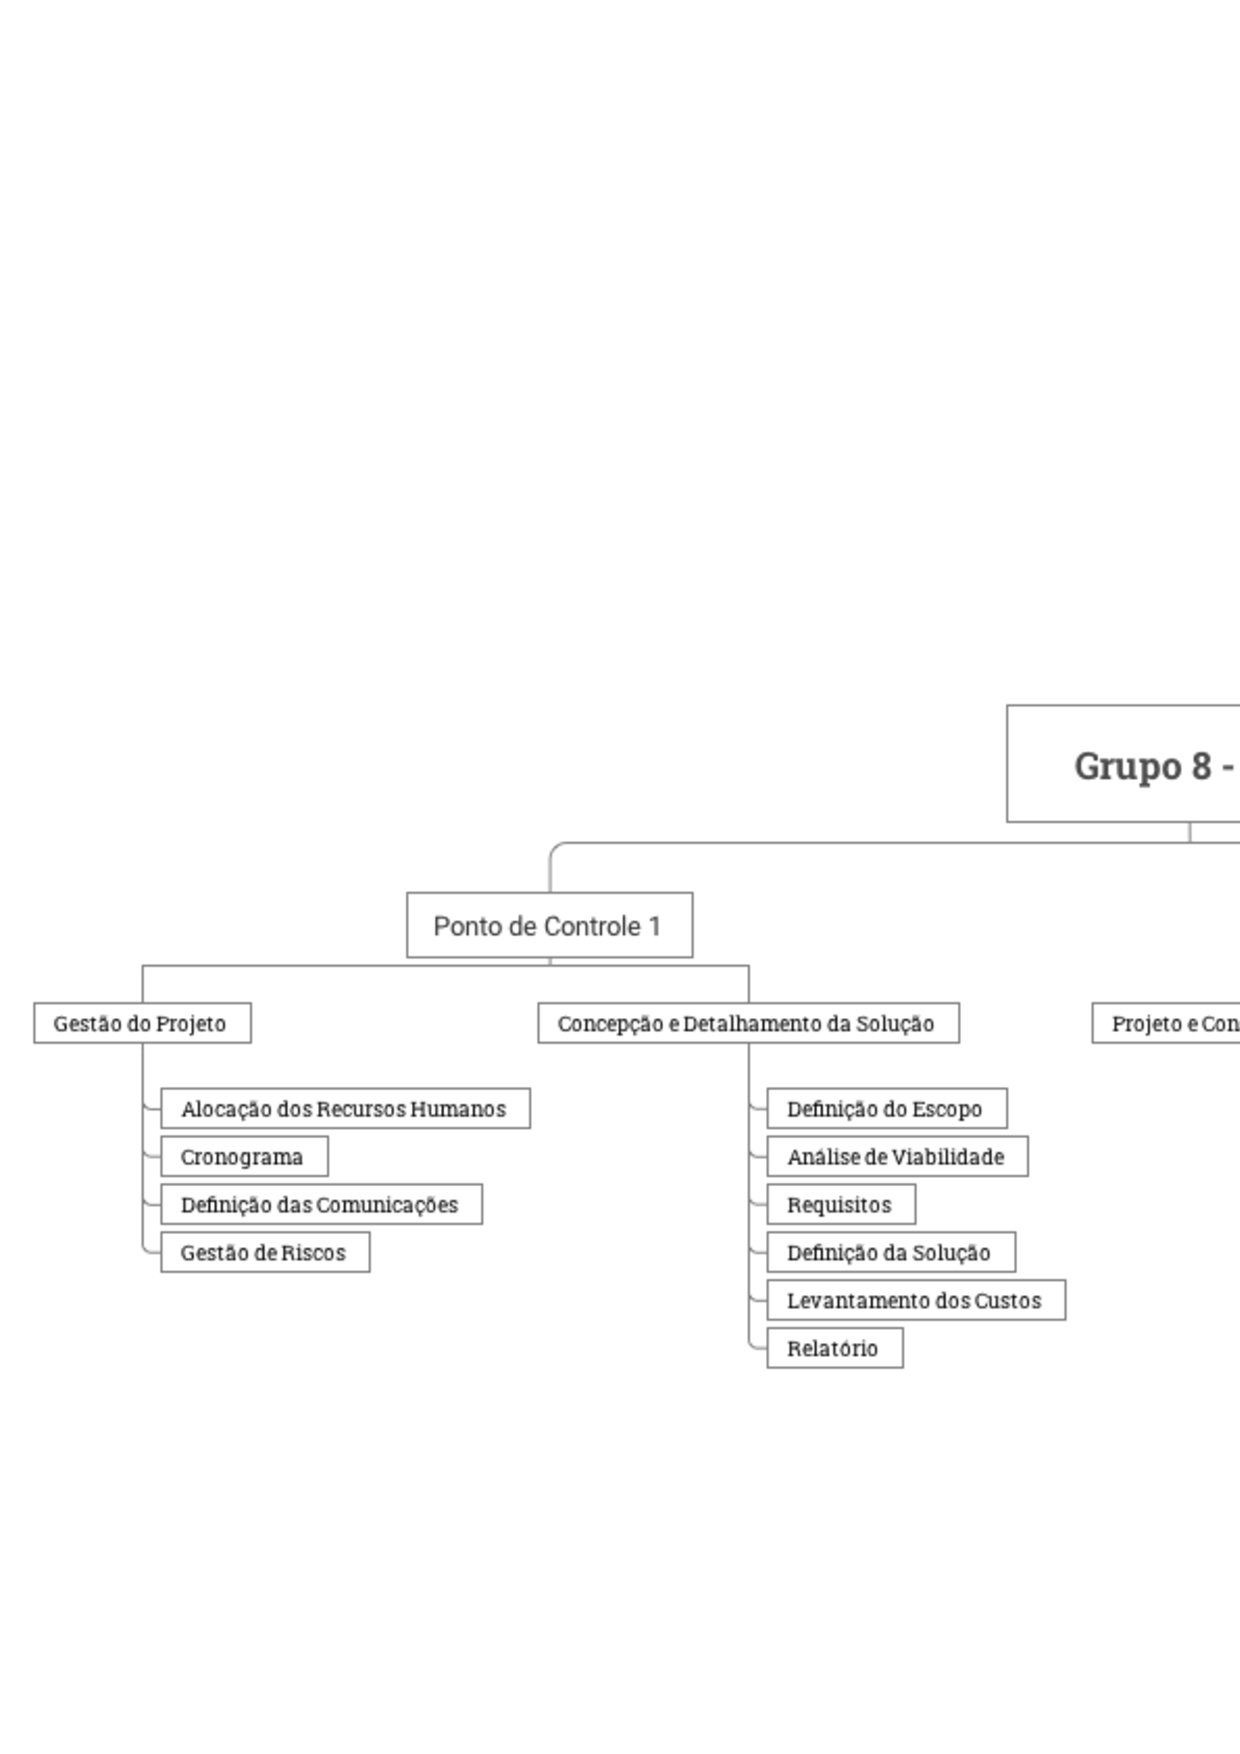
\includegraphics[width=\textwidth]{figuras/EAP.png}
\caption{\label{fig:eap}Estrutura Analítica do Projeto.}
\end{center}
\end{figure}

    \subsection{Alocação dos Recursos Humanos}

A equipe do projeto, formada por 15 (quinze) integrantes, foi
subdivida em 4 (quatro) áreas de atuação, que são elas: "Controle
e Sensoriamento", "Localização no Ambiente e Informações", "Perfuração
e Coleta" e "Tração, Energia Utilizada e Estrutura". As áreas são
supervisionadas e administradas por uma gestora geral, Jéssica Guimarães,
e por um gestor de qualidade, Leonardo Cambraia.

Cada uma das áreas acima citadas é responsável pela análise de alternativas
para a solução e a escolha de uma destas para ser aplicada no projeto.

A figura \ref{fig:aloc} ilustra a estrutura de alocação de recursos humanos do
projeto. A divisão dos integrantes foi feita levando-se em conta o
interesse de cada um nas áreas propostas e o conhecimento prévio de
cada um. É importante salientar que toda a estrutura está sujeita a
mudanças, sempre visando o suprir bem as necessidades do projeto.

\begin{figure}[!htbp]
\begin{center}
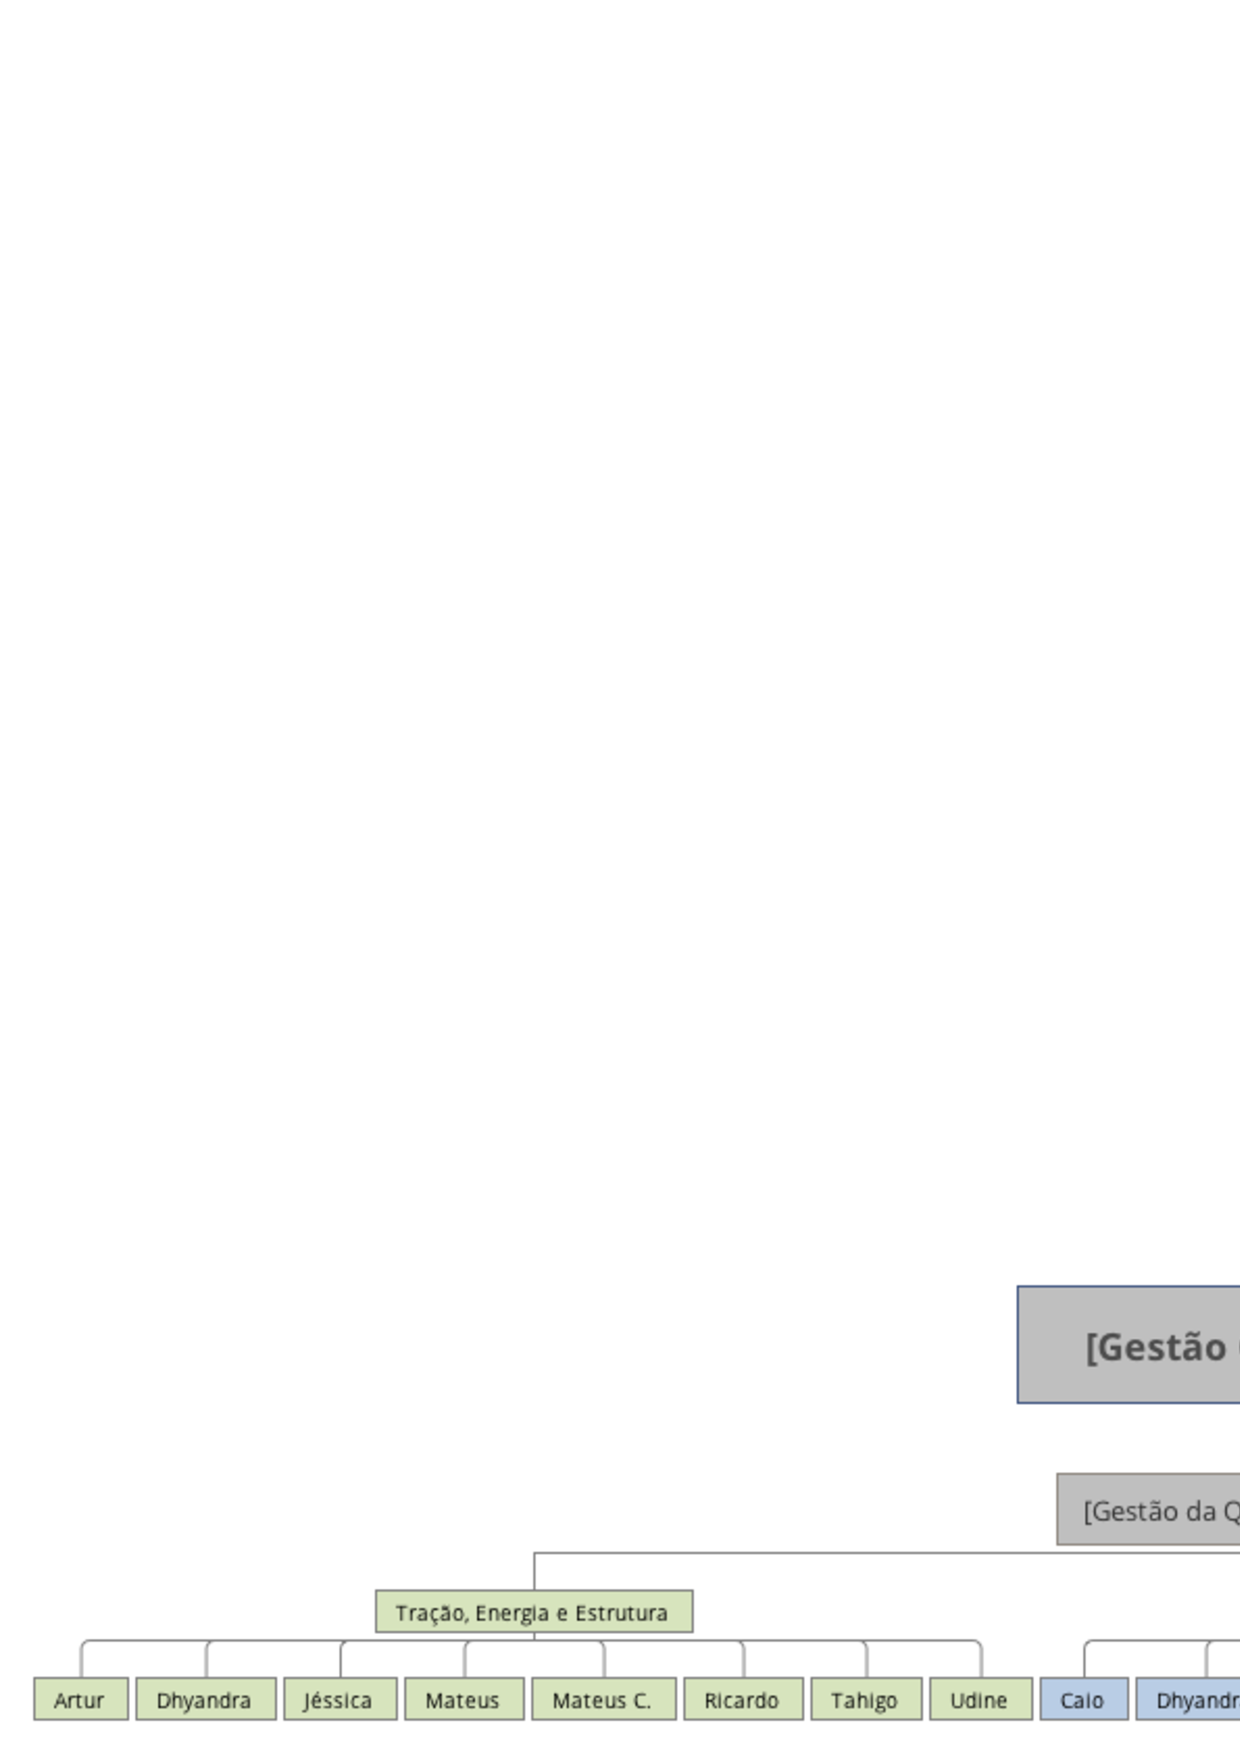
\includegraphics[width=\textwidth]{figuras/alocacao.png}
\caption{\label{fig:aloc}Alocação de recursos humanos.}
\end{center}
\end{figure}

    \subsection{Comunicação}

O sucesso de todo projeto é diretamente relacionado ao engajamento
da equipe, sendo que para isso é necessária boa comunicação entre os
membros da equipe. A tabela \ref{tab:com} detalha os métodos de comunicação
utilizados pela equipe.

\begin{table}[!htbp]
\begin{center}
\begin{tabular}{|p{4cm}|p{4cm}|p{3cm}|p{3cm}|p{2cm}|}
\hline
\textbf{Objetivos} & \textbf{Ferramenta} & \textbf{Frequência} & \textbf{Horário} & \textbf{Local}\\\hline
Acompanhamento das atividades & Trello & Sob demanda & N/A & N/A\\\hline
Avisos rápidos / Lembretes & Telegram & Sob demanda & N/A & N/A\\\hline
Decisões Técnicas/Planejamentos & Presencial & Duas vezes por semana & Horário da disciplina & FGA\\\hline
Desenvolvimento do projeto & Google Docs/ Google Hangouts/ Presencial & Sob demanda & À definir & À definir\\\hline
\end{tabular}
\caption{\label{tab:com}Métodos de comunicação.}
\end{center}
\end{table}

    \subsection{Tempo}

Para a definição das atividades a serem realizadas durante o
projeto utilizou-se como base os pacotes de trabalho estabelecidos
na Estrutura Analítica do Projeto (EAP), onde os mesmos foram devidamente
decompostos com base nos três grandes marcos do projeto referentes
às entregas de Ponto de Controle 1, 2 e 3. Para tal feito, a equipe,
tanto de gerência quanto de desenvolvimento precisará cumprir
as atividades elucidadas no cronograma.

Após decompostos os pacotes de trabalho da EAP, a equipe
de gerência reuniu-se para discutir como suas atividades seriam
executadas, visando tanto uma paralelização de atividades quanto
o tempo estimado e os recursos necessários para tal.

Para a determinação do tempo foi utilizado foram utilizadas as
técnicas de \textbf{Analogia} e \textbf{Decisão em Grupo},
as quais, segundo o \cite{PMI2012}, representam:
\begin{itemize}
\item Analogia: baseia-se em pacotes de trabalho/atividades similares
de projetos anteriores para estimar a duração dos pacotes de trabalho
e/ou atividades do seu projeto atual.
\item Decisão em Grupo: nessa técnica o envolvimento da equipe de projeto
nas estimativas proporcionam maior comprometimento da mesma com as
atividades a serem realizadas.
\end{itemize}

O cronograma referente ao nosso projeto encontra-se na figura \ref{fig:cron_s1}
abaixo, contendo seus pacotes de trabalho, atividades e datas. Outro
cronograma mais detalhado está disposto no Anexo X. (Arquivo no Drive)

\begin{figure}[!htbp]
\begin{center}
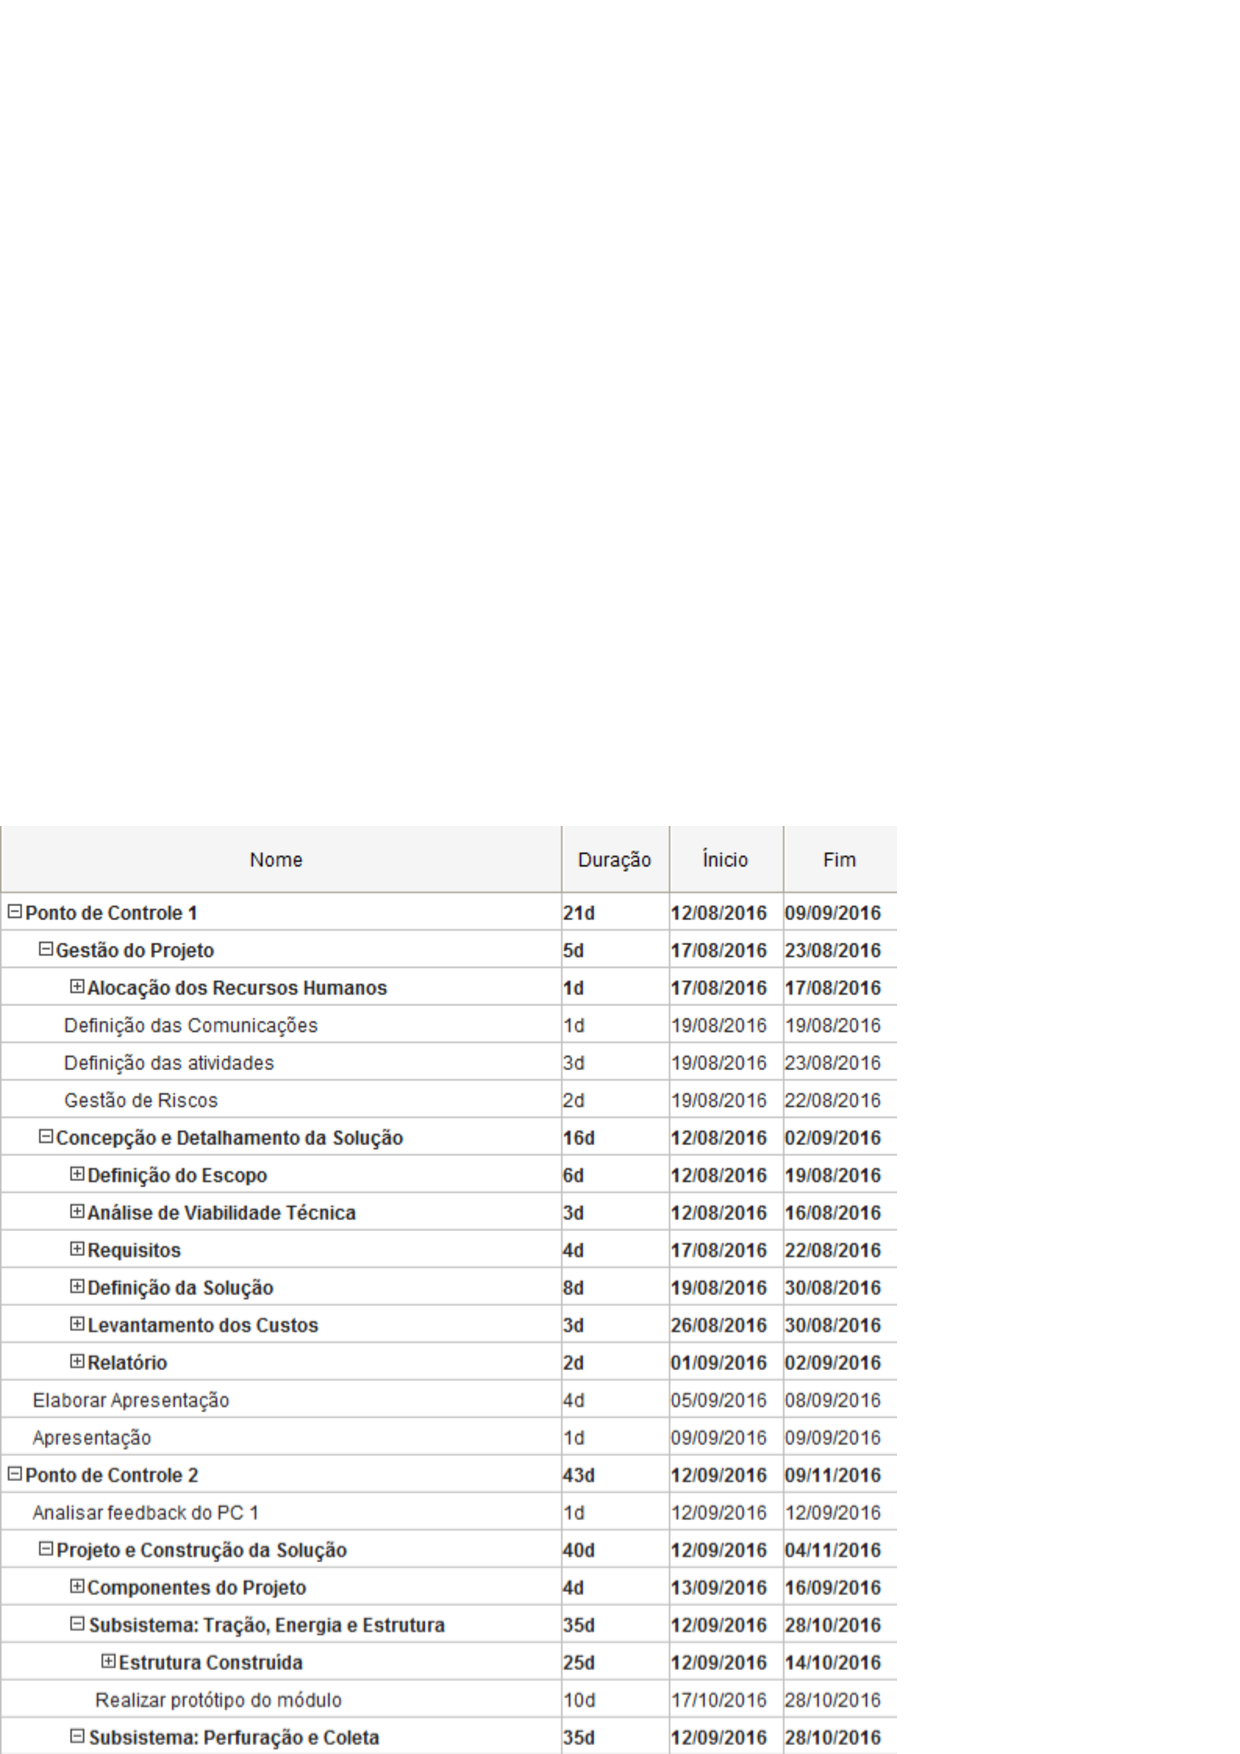
\includegraphics[width=\textwidth]{figuras/cronograma_simples_1.png}
\caption{\label{fig:cron_s1}Cronograma de Atividades simplificado (parte 1).}
\end{center}
\end{figure}

\begin{figure}[!htbp]
\begin{center}
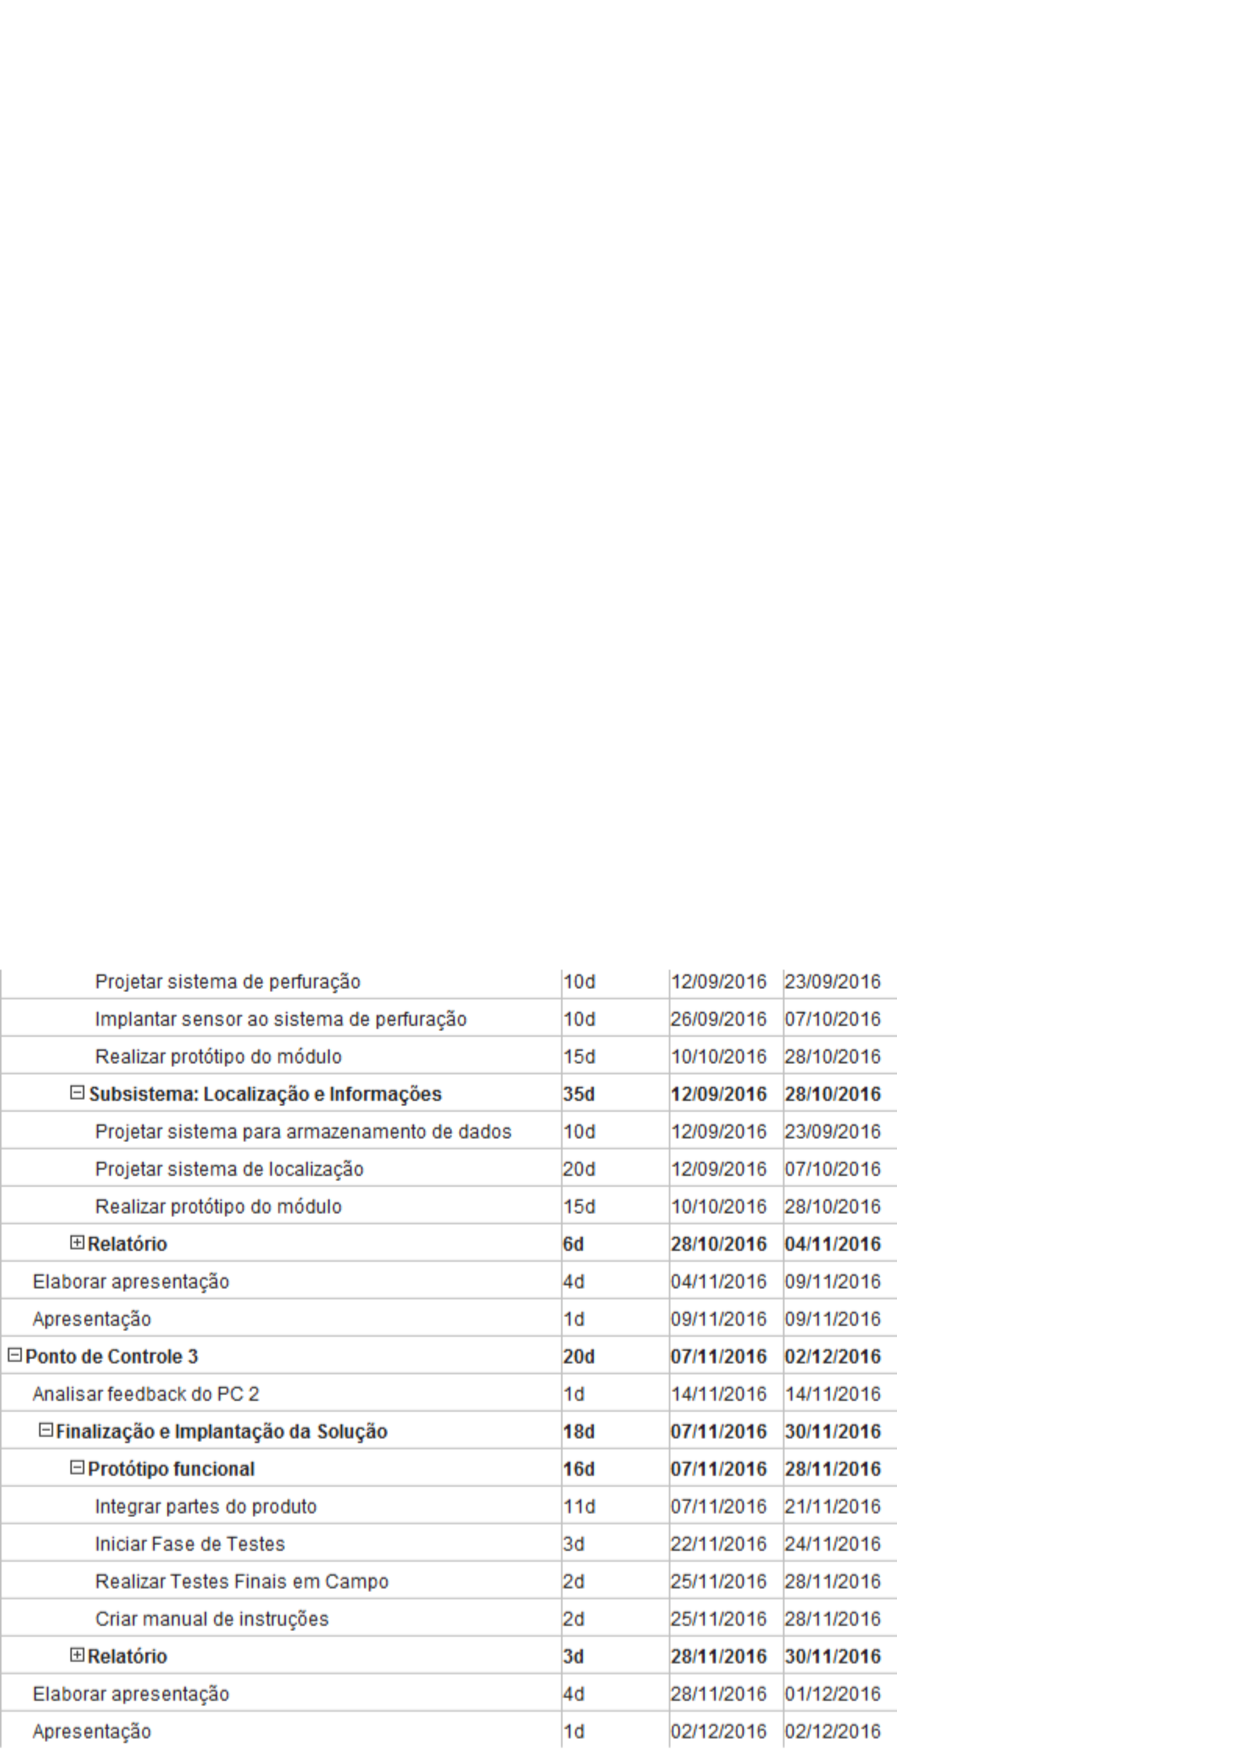
\includegraphics[width=\textwidth]{figuras/cronograma_simples_2.png}
\caption{\label{fig:cron_s2}Cronograma de Atividades simplificado (parte 2).}
\end{center}
\end{figure}

  \section{Riscos}
  
